\documentclass[de]{./../../common/SurferDesc}%%%%%%%%%%%%%%%%%%%%%%%%%%%%%%%%%%%%%%%%%%%%%%%%%%%%%%%%%%%%%%%%%%%%%%%
%
% The document starts here:
%
\begin{document}
\footnotesize
% Weltrekordfl�chen

%%% 1.Tafel

%%%%%%%%%%%%%%%%%%%%%%%%%%%%%

\begin{surferPage}
  \begin{surferTitle}Barths Sextik mit 30 Cuspen\end{surferTitle}  

    Nachdem Wolf Barth seine Sextik mit der maximal m�glichen Anzahl von $65$
    Singularit�ten gefunden hatte
    und zwei seiner Doktoranden ebenfalls neue Weltrekorde f�r h�here Grade
    aufgestellt hatten, besch�ftigt er sich auch mit der Frage nach der
    maximal m�glichen Anzahl von Kuspen auf Fl�chen von gegebenem Grad. 

    Barths Kontruktion der Sextik mit $65$ 
    Singularit�ten vom Typ $A_1^{+-}$ (also Doppelkegel) kann man auf Kuspen
    adaptieren (allerdings nur $30$ St�ck):
    \[P_6 - \alpha \cdot K^3=0,\]
    wobei $P_6$ wie bei der anderen Barth-Sextik die Symmetrieebenen des
    regelm��igen Ikosaeders sind und $K$ die Gleichung einer Kugeloberfl�che
    ist:
    \vspace*{-0.4em}
    \begin{center}
      \begin{tabular}{c@{\ }c@{\ }c@{\ }c}
        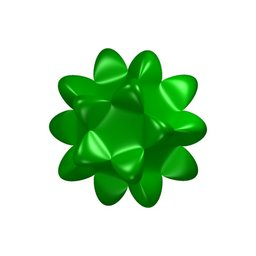
\includegraphics[height=1.2cm]{./../../common/images/barthsextic_30A2}
        &
        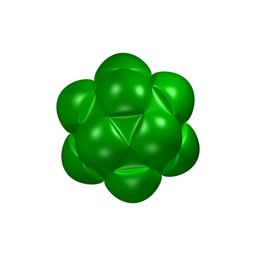
\includegraphics[height=1.2cm]{./../../common/images/barthsextic_30A2_3}
        &
        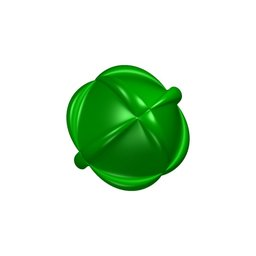
\includegraphics[height=1.2cm]{./../../common/images/barthsextic_30A2_5}
        &
        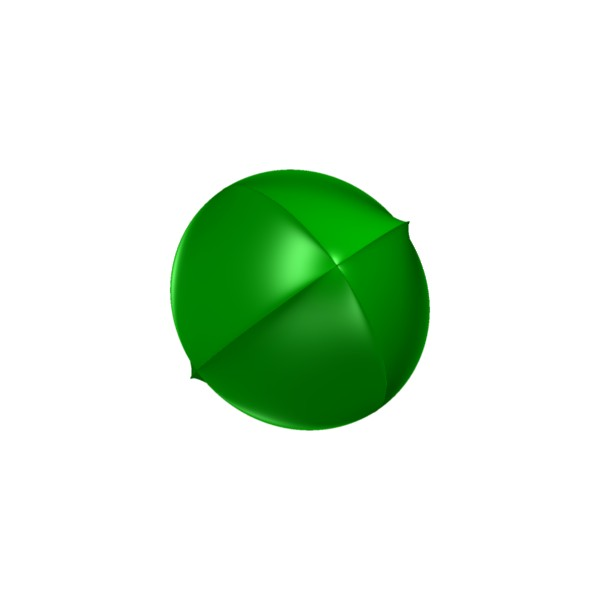
\includegraphics[height=1.2cm]{./../../common/images/barthsextic_30A2_6}
      \end{tabular}
    \end{center}    
    \vspace*{-0.3em}
    Dies ist der aktuelle Weltrekord f�r die maximale Anzahl reeller Kuspen
    auf Sextiken, f�r komplexe liegt er bei $36$. 



  \begin{surferText}
     \end{surferText}
\end{surferPage}
%%%%%%%%%%%%%%%%%%%%%%%%%%%%%


\end{document}
%
% end of the document.
%
%%%%%%%%%%%%%%%%%%%%%%%%%%%%%%%%%%%%%%%%%%%%%%%%%%%%%%%%%%%%%%%%%%%%%%%
